% !TeX root = ../b01.tex

\section{Aufgabe BI-2}

\begin{task}
    Für die Bevölkerung gewisser Regionen der Erde wurden folgende Geschlechterverteilungen (das heißt Männer 100 Frauen)
    \begin{tightcenter}
        96  101  98  96  101  98  105  106  101  104  88  97 \\
        100  96  101  92  98  104  102  97  98  93  100  94
    \end{tightcenter}
    durch statistische Erhebungen erhalten.

    \begin{enumerate}
        \item[(a)] Stellen Sie die Daten in einem Histogramm mit 5 Klassen gleicher Klassenbreite dar.
    \end{enumerate}
\end{task}

geordnete Urliste: 88 92 93 94 96 96 96 97 97 98 98 98 98 100 100 101 101 101 101 102 104 104 105 106

Stichprobenumfang $n=24$

$\sqrt{n} = \sqrt{24} \approx 4.8990 \Rightarrow \ell=5$ Klassen (nach Faustregel)

Einteilung der Klassen mit Breite $d_j=5$ wie folgt:

\begin{table}[H]
\centering
\begin{tabular}{c|ccccc}
    $j$                       & 1                   & 2         & 3          & 4                  & 5                   \\ \hline
    Klasse                    & $[85,90)$           & $[90,95)$ & $[95,100)$ & $[100,105)$        & $[105,110)$         \\
    absolute Häufigkeit $h_j$ & 1                   & 3         & 9          & 10                 & 1                   \\
    relative Häufigkeit $r_j$ & $0.041\overline{6}$ & 0.125     & 0.375      & $0.41\overline{6}$ & $0.041\overline{6}$
\end{tabular}
\end{table}

\begin{figure}[H]
    \centering
    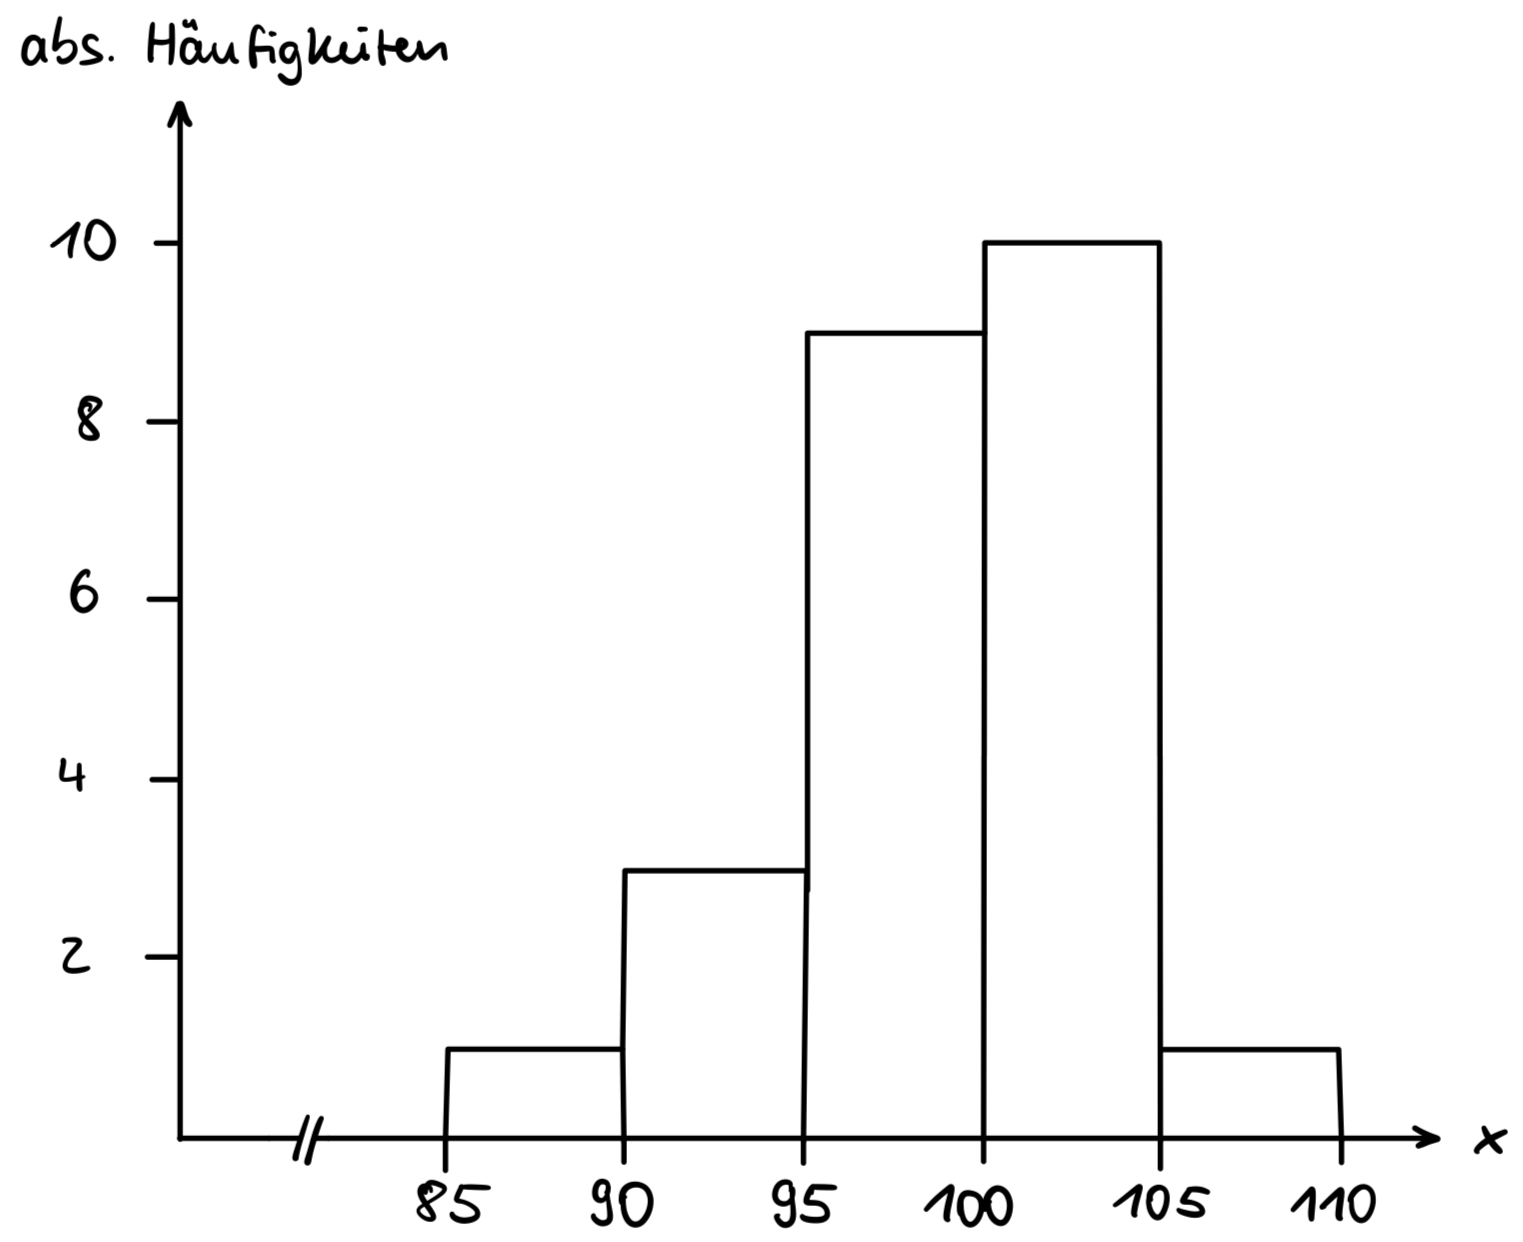
\includegraphics[width=0.8\textwidth]{assets/task2_histogramm.jpeg}
    \caption{Histogramm für Aufgabe 2.a (handgezeichnet)}
\end{figure}

\begin{figure}[H]
    \centering
    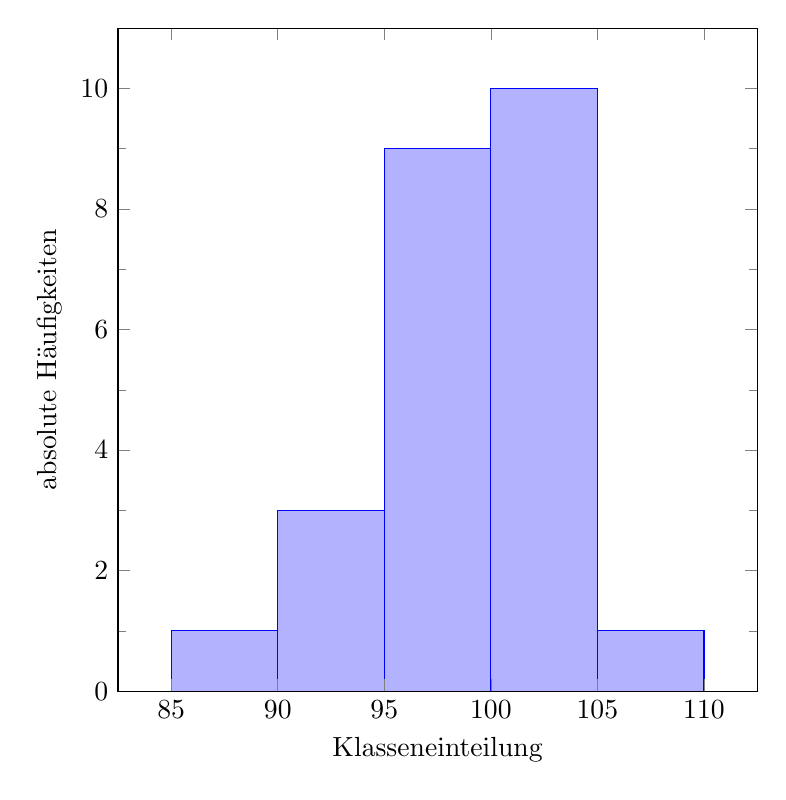
\begin{tikzpicture}
    \begin{axis}[
        width=0.8\textwidth, height=10cm,
        area style,
        ymin=0, ymax=11,
        ylabel = absolute Häufigkeiten,
        xlabel = Klasseneinteilung,
        ytick distance=2,
        minor y tick num = 1,
        xtick distance=5
    ]
        \addplot+[ybar interval, mark=no] plot coordinates { (85,1) (90,3) (95,9) (100,10) (105,1) (110,0)};
    \end{axis}
    \end{tikzpicture}
    \caption{Histogramm für Aufgabe 2.a (PGF/TikZ)}
\end{figure}


\begin{task}
    \begin{enumerate}
        \item[(b)] Berechnen Sie die Werte der (gewöhnlichen, nicht klassierten) empirischen Verteilungsfunktion $F$ der Daten an den Stellen $x_1=95.5$ und $x_2=100$.
    \end{enumerate}
\end{task}

% ACHTUNG: **NICHT** klassiert!!

\begin{table}[H]
\centering
\begin{tabular}{c|clll}
     $j$      & $a_j$ & $h_j$     & $r_j$               & $F(x_j)$ \\ \hline
     1        & 88    & 1         & $0.041\overline{6}$ & $0.041\overline{6}$ \\
     2        & 92    & 1         & $0.041\overline{6}$ & $0.08\overline{3}$  \\
     3        & 93    & 1         & $0.041\overline{6}$ & $0.125$             \\
     4        & 94    & 1         & $0.041\overline{6}$ & $0.1\overline{6}$   \\
     5        & 96    & 3         & $0.125$             & $0.291\overline{6}$ \\
     6        & 97    & 2         & $0.08\overline{3}$  & $0.375$             \\
     7        & 98    & 4         & $0.1\overline{6}$   & $0.541\overline{6}$ \\
     8        & 100   & 2         & $0.08\overline{3}$  & $0.625$             \\
     9        & 101   & 4         & $0.1\overline{6}$   & $0.791\overline{6}$ \\
     $\vdots$ & $\vdots$ & $\vdots$  & $\vdots$            & $\vdots$
\end{tabular}
\end{table}

$$
F(x) = \begin{cases}
    0      & \text{für}~x<88 \\
    % 0.0417 & \text{für}~88\le x<92 \\
    % 0.0833 & \text{für}~92\le x<93 \\
    % 0.125  & \text{für}~93\le x<94 \\
    \vdots & \\
    0.1\overline{6} & \text{für}~94\le x<96 \\
    \vdots & \\
    % 0.2917 & \text{für}~96\le x<97 \\
    % 0.375  & \text{für}~97\le x<98 \\
    % 0.5417 & \text{für}~98\le x<100 \\
    0.625  & \text{für}~100\le x<101 \\
    \vdots & \\
    1      & \text{für}~x\le 106
\end{cases}
$$

$\Rightarrow F(x_1) = F(95.5) = 0.1\overline{6},~~F(x_2) = F(100) = 0.625$

Die empirische Verteilungsfunktion nimmt an der Stelle $x_1=95.5$ den Wert $0.1\overline{6}$ und an der Stelle $x_2=100$ den Wert $0.625$ an.


\begin{task}
    \begin{enumerate}
        \item[(c)] Erstellen Sie den zu den Beobachtungswerten gehörigen klassischen Box-Plot (mit Kennzeichnung von Ausreißern und Extremwerten, so vorhanden).
    \end{enumerate}
\end{task}

Fünf-Punkte-Zusammenfassung

$x_{(1)} = 88$

$q\cdot n = 0.25\cdot 24 = 6\in\mathbb{Z} \Rightarrow$ nicht eindeutig \\
$\Rightarrow \tilde{x}_{0.25} = \frac12(x_{(6)} + x_{(7)}) = \frac12(96+96) = 96$

$n = 24 \notin 2\mathbb{N}$ \\
$\Rightarrow x_{\operatorname{med}} = \frac12(x_{(12)} + x_{(13)}) = \frac12(98+98) = 98$

$q\cdot n = 0.75\cdot 24 = 18\in\mathbb{Z} \Rightarrow$ nicht eindeutig \\
$\Rightarrow \tilde{x}_{0.75} = \frac12(x_{(18)} + x_{(19)}) = \frac12(101+101) = 101$

$x_{(n)} = x_{(24)} = 106$

\vspace{0.5cm}

$\Rightarrow$ Quartilsabstand $d_Q = \tilde{x}_{0.75} - \tilde{x}_{0.25} = 101 - 96 = 5$

$\frac32 \cdot d_Q = \frac32\cdot5 = 7.5 \Rightarrow [88.5, 108.5]$ \\
$\Rightarrow$ Ausreißer: $\lbrace 88 \rbrace$

$3\cdot d_Q = 3\cdot5 = 15 \Rightarrow [81, 116]$ \\
$\Rightarrow$ keine Extremwerte

\vspace{0.5cm}

linker Whisker: $\min\lbrace x_j : x_j \ge \tilde{x}_{0.25} - \frac32 d_Q \rbrace = 92$

rechter Whisker: $\max\lbrace x_j : x_j \le \tilde{x}_{0.75} + \frac32 d_Q \rbrace = 106$

\begin{figure}[H]
    \centering
    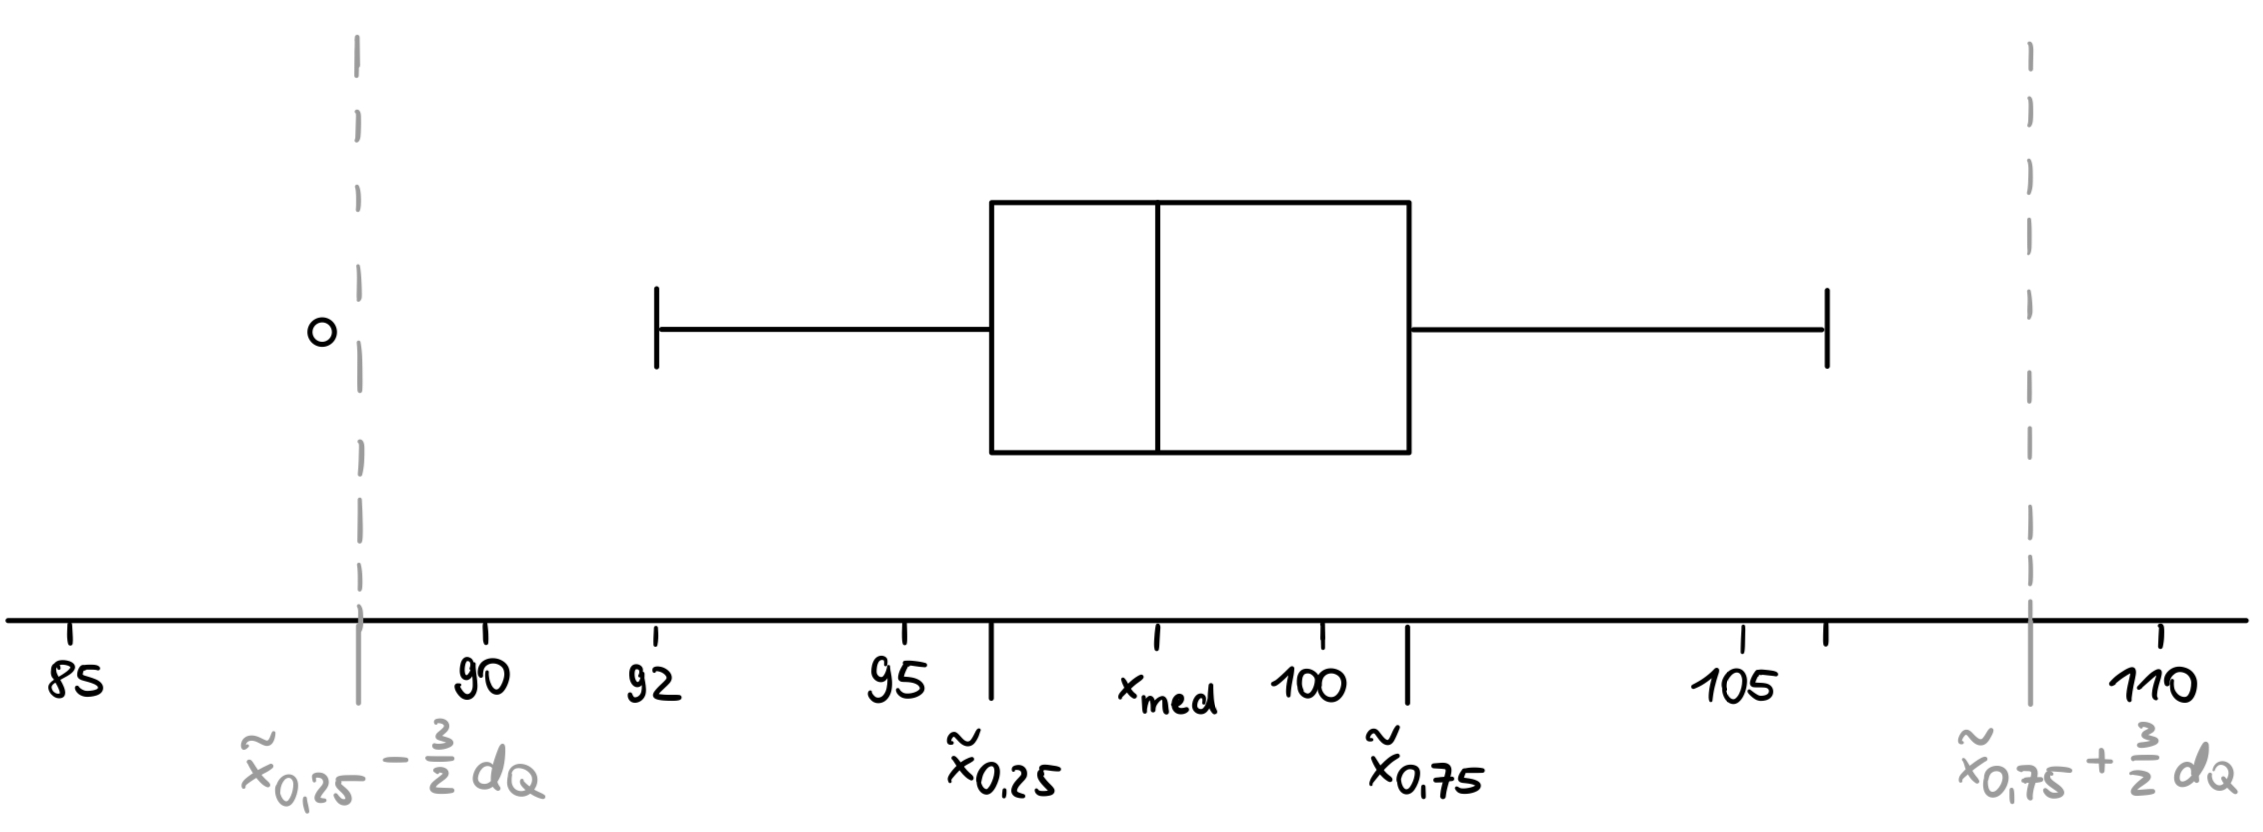
\includegraphics[width=\textwidth]{assets/task2_box_plot.jpeg}
    \caption{Klassischer Box-Plot zu Aufgabe 2.c (handgezeichnet)}
\end{figure}

\begin{figure}[H]
    \centering
    \begin{tikzpicture}
    \begin{axis}[
        width=0.9\textwidth, height=5cm,
        xmin=80, xmax=120,
        ymin=0, ymax=2, yticklabel=\empty
    ]
        \addplot+[
            boxplot prepared={
                median=98,
                upper quartile=101,
                lower quartile=96,
                upper whisker=92,
                lower whisker=106
            }
        ] coordinates { (0,88) };   % Ausreißer

        \addplot[dashed] coordinates {(88.5,0) (88.5,2)};
        \addplot[dashed] coordinates {(108.5,0) (108.5,2)};
        
        \addplot[dashed] coordinates {(81,0) (81,2)};
        \addplot[dashed] coordinates {(116,0) (116,2)};
    \end{axis}
    \end{tikzpicture}
    \caption{Klassischer Box-Plot zu Aufgabe 2.c (PGF/TikZ)}
\end{figure}
